\documentclass[11pt]{amsart} %amscd adds the macros for the commutative diagram environment

\usepackage{fullpage, amsmath, amssymb, amsthm, enumitem, tabularx, multirow, multicol, tikz, venndiagram, graphicx, caption, xcolor, array, tabularx, wrapfig, nicefrac}
\renewcommand{\baselinestretch}{1.15}

\theoremstyle{plain}
\newtheorem{thrm}{Theorem}

\theoremstyle{definition}
\newtheorem*{dfn}{Definition}

\theoremstyle{definition}
\newtheorem*{prpn}{Proposition}

\theoremstyle{remark}
\newtheorem*{note}{Note}

\theoremstyle{definition}
\newtheorem*{lemma}{Lemma}

\usepackage{Sweave}
\begin{document}
\Sconcordance{concordance:Math_Concepts_3a_LinearAlgebra.tex:Math_Concepts_3a_LinearAlgebra.Rnw:1 %
20 1 1 0 122 1}


\title{\underline{Math Concepts 3} \\
        Linear Algebra: \\
        \emph{Vectors}}

\author{Emre Usenmez}

\thanks{These notes made liberal use of the following books Johnston, N (2021) \textit{Introduction to Linear and Matrix Algebra} Springer DOI: 10.1007/978-3-030-52811-9; Hefferon, J (2020) \textit{Linear Algebra} 4th ed, available at: http://joshua.smcvt.edu/linearalgebra; Vinod H D (2011) \textit{Hands-On Matrix Algebra Using R} World Scientific; and Deisenroth, M P, Faisal, A A, and Ong C S (2020) \textit{Mathematics for Machine Learning} CUP.}
%\date{August 2023}

\maketitle

\section{Vectors and Vector Operations}

\noindent
\begin{wrapfigure}{r}{0.25\textwidth}
      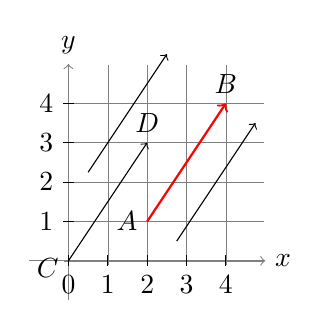
\begin{tikzpicture}
            \draw [thin, gray, ->, scale=0.5] (0,-1) -- (0,5) node [above, black] {$y$};
            \draw [thin, gray, ->, scale = 0.5] (-1,0) -- (5,0) node [right, black] {$x$};
            \draw[step=0.5cm, gray, very thin](-0.05,-0.05) grid (2.49,2.49);
            \foreach \y in {1,2,3,4}
                    \draw (2pt, \y*0.5cm) -- (-2pt, \y*0.5cm) node[left]{$\y$};
            \foreach \x in {0,1,2,3,4}
                    \draw (\x*0.5cm,2pt) --(\x*0.5cm,-2pt) node[below]{$\x$};
            \draw [draw=red, thick, scale=0.5, ->] (2,1) -- (4,4);
                  \node [left] at (1,0.5) {$A$};
                  \node [above] at (2,2) {$B$};
            \draw[scale=0.5, ->](0,0)--(2,3);
                  \node [below left] at (0,0.15) {$C$};
                  \node [above] at (1,1.5) {$D$};
            \draw[scale=0.5, ->](2.75,0.5)--(4.75, 3.5);
            \draw[scale=0.5, ->](0.5,2.25)--(2.5,5.25);
      \end{tikzpicture}
\end{wrapfigure}

The head of a vector is where the tip of the arrow is and its tail is where it begins at the opposite end of the arrow. On the graph to the left we have point $A$ located at (2,1) and point $B$ located at (4,4). The vector joining the two dots is $\overrightarrow{AB}$ which can be represented as a set of two numbers that indicate the distance $x$ and $y$ travels: (4,4) - (2,1) = (2,3). However, (2,3) is the same vector as all the other vectors shown in the graph. This is why it is good to think vectors as \emph{displacements.}

\medskip

This vector is a displacement of "two over and three up". Wherever they start, they displace by "two over and three up". This is why they are called \emph{free} vectors. These vectors are not similar nor alike, they are \emph{equal}. Generally, vectors are the same if and only if the changes in their individual components are the same. That is, a vector $\vec{v}$ extending from $(a_1, a_2)$ to $(b_1, b_2)$ is equal to vector $w$ extending from $(c_1, c_2)$ to $(d_1, d_2)$ if and only if the change in the first component of $\vec{v}$, $b_1 - a_1$ is equal to the change in the first component of $\vec{w}$, $d_1 - c_1$, as well as if the change in their second components are the same, i.e., $b_2 - a_2 = d_2 - c_2$. That is, $\vec{v} = \vec{w}$ if and only if

\begin{displaymath}
    \begin{pmatrix}
          b_1 - a_1 \\
          b_2 - b_2
    \end{pmatrix}
=
    \begin{pmatrix}
        d_1 - c_1 \\
        d_2 - c_2
    \end{pmatrix}
\end{displaymath}

\medskip
It should be noted that the coordinates of a vector, such as (2,3), specify its length and direction. It does not tell us its location in space. Vectors can be moved around in space without changing the vector itself. To remove this ambiguity about its location, vectors are often drawn as starting at the origin, like the vector $\overrightarrow{CD}$ in the graph above where it is in its \emph{canonical position}. Textbooks also refer to this as \emph{natural position} or \emph{standard position.}

We can also think of vector $\overrightarrow{CD}$ representing $\{(0,0) + (2,3)t : t\in\mathbb{R}\}$ and vector $\overrightarrow{AB}$ representing $\{(2,1) + (2,3)t : t\in\mathbb{R}\}$.


\medskip
Similarly, in $\mathbb{R}^{3}$, the line through (3,1,2) and (0,2,4) is the set of vectors $\{ \left( \begin{smallmatrix}3 \\ 1 \\ 2\end{smallmatrix} \right) + t\cdot \left( \begin{smallmatrix}-3 \\ -1 \\ -2\end{smallmatrix} \right) : t\in\mathbb{R} \}$; and the plane through the points (1,2,3), (-2,4,-6), and (1,-3,5) consists of the vectors in this set $\{ \left( \begin{smallmatrix} 1 \\ 2 \\ 3 \end{smallmatrix} \right) + t \cdot \left( \begin{smallmatrix} -3 \\ 2 \\ -9 \end{smallmatrix} \right) + s \cdot \left( \begin{smallmatrix} 0 \\ -5 \\ 2 \end{smallmatrix} \right) : s,t\in\mathbb{R} \}$.

\begin{note}
Notice that the vectors associated with the parameters $s$ and $t$ are determined in relation to the particular point (1,2,3). This is because a particle would be free to move on the plane in a combination of two directions. In this sense, the parameters for $s$ and $t$ are unrestricted, whereas (1,2,3) is restricted to that point.
\end{note}

\medskip
Books usually describe a plane with a linear equation $Plane = \{ \left( \begin{smallmatrix} x \\ y \\ z \end{smallmatrix} \right) : 4x -  3y + 2z = 12 \}$. In order to translate this to the vector description we can think of this as a linear system and parametrize it: $x = 3 + \frac{3}{4}y - \frac{1}{2}z$. Therefore, $Plane = \{ \left( \begin{smallmatrix} 3 \\ 0 \\ 0 \end{smallmatrix} \right) + y \cdot \left( \begin{smallmatrix} \nicefrac{3}{4} \\ 1 \\ 0 \end{smallmatrix} \right) + z \cdot \left( \begin{smallmatrix} \nicefrac{1}{2} \\ 0 \\ 1 \end{smallmatrix} \right) : y,z\in\mathbb{R} \}$.


\medskip
If we generalize this, then a set of the form $\{ \vec{p} + t_1\vec{v_1} + t_2\vec{v_2} +\dots+ t_k\vec{k} : t_1,\dots,t_k \in\mathbb{R} \}$ where $\vec{v_1},\dots,\vec{v_k} \in\mathbb{R}^{n}$ and $k\leq n$ is a \emph{k-dimensional linear surface}, or \emph{k-flat}.

\smallskip
For example, in $\mathbb{R}^{4}$, $\{ \left( \begin{smallmatrix} 1 \\ 2 \\ 3 \\ 4 \end{smallmatrix} \right) + t \cdot \left( \begin{smallmatrix} 7 \\ -2 \\ 13 \\ 0 \end{smallmatrix} \right) : t \in\mathbb{R}\}$ is a line, whereas $\{ \left( \begin{smallmatrix} 0 \\ 0 \\ 0 \\ 0 \end{smallmatrix} \right) + t \cdot \left( \begin{smallmatrix} 1 \\ -1 \\ 1 \\ -1 \end{smallmatrix} \right) + s \cdot \left( \begin{smallmatrix} 2 \\ 2 \\ 0 \\ 2 \end{smallmatrix} \right) : t,s \in\mathbb{R} \}$ is a plane, and $\{ \left( \begin{smallmatrix} -2 \\ 0 \\ -7 \\ 3 \end{smallmatrix} \right) + t \cdot \left( \begin{smallmatrix} 1 \\ 2 \\ 3 \\ 4 \end{smallmatrix} \right) + s \cdot \left( \begin{smallmatrix} -3.5 \\ 5 \\ 5 \\ 1 \end{smallmatrix} \right) + r \cdot \left( \begin{smallmatrix} 0 \\ 2 \\ 3 \\ 0 \end{smallmatrix} \right) : t,s,r \in\mathbb{R} \}$ is a three dimensional linear surface.
\smallskip
When the dimension of the linear surface is one less than the dimension of the space like the three-flat in $\mathbb{R}^{4}$ above, that is, when in $\mathbb{R}^{n}$ we have an (n-1)-flat, that surface is called a \emph{hyperplane}.



\bigskip
\begin{wrapfigure}{r}{0.35\textwidth}
      \begin{tabular}{r r}
            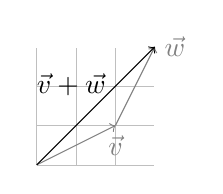
\begin{tikzpicture}
                  \draw[step=0.5cm, gray!50, very thin](0,0) grid (1.49,1.49);
                  \draw[thin, gray, ->] (0,0)--(1,0.5) node[below] {$\vec{v}$};
                  \draw[thin, gray, ->] (1,0.5)--(1.5,1.5) node[right]{$\vec{w}$};
                  \draw[->] (0,0)--(1.5, 1.5) node[above left] at (1,0.75) {$\vec{v}+\vec{w}$};
            \end{tikzpicture}
            &
            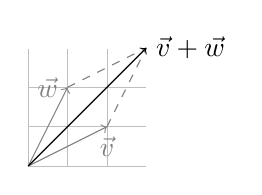
\begin{tikzpicture}
                  \draw[step=0.5cm, gray!50, very thin](0,0) grid (1.49,1.49);
                  \draw[thin, gray, ->] (0,0)--(1,0.5) node[below] {$\vec{v}$};
                  \draw[thin, gray, ->] (0,0)--(0.5,1) node[left] {$\vec{w}$};
                  \draw[thin, gray, dashed, -] (1,0.5)--(1.5,1.5);
                  \draw[thin, gray, dashed, -] (0.5,1)--(1.5,1.5);
                  \draw[->] (0,0)--(1.5,1.5) node[right] at (1.5, 1.5) {$\vec{v}+\vec{w}$};
            \end{tikzpicture}
      \end{tabular}
\end{wrapfigure}
      In general, if we see $\vec{v}$ and $\vec{w}$ as displacements, then $\vec{v}+\vec{w}$ is a combined displacement. This can be represented geometrically in two different ways: either as a head-to-tail or in standard position with the parallelogram rule as shown on the right.


\begin{thrm}
      Suppose $\vec{v}, \vec{w}, \vec{x} \in\mathbb{R}^{n}$ are vectors. Then the following properties hold:
      \begin{enumerate}
            \item[i] Commutativity: $\vec{v}+\vec{w} = \vec{w}+\vec{v}$
            \item[ii] Associativity: $(\vec{v}+\vec{w})+\vec{x} = \vec{v}+(\vec{w}+\vec{x})$.
      \end{enumerate}
\end{thrm}

\begin{proof}
      To prove part (i) we will make use of the definition of vector addition and the fact that addition of real numbers is commutative:
      \[
                \vec{v}+\vec{w} = (v_1+w_1, v_2+w_2,\dots,v_n+w_n)
                = (w_1+v_1, w_2+v_2, \dots, w_n+v_n) = \vec{w}+\vec{v}.
           \]
      Proof of part (ii) follows a similar pattern making use of the definition of vector addition and the property of real number addition.
\end{proof}


Another basic operation on vectors called \emph{scalar multiplication} changes a vector's length and can reverse its direction.

\begin{dfn}
      Suppose $\vec{v} = (v_1, v_2,\dots,v_n) \in\mathbb{R}^{n}$ and $c\in\mathbb{R}$, is a scalar. Then the \emph{scalar multiplication} of real number $c$ and vector $\vec{v}$ is:
      \[ c\vec{v}= c \cdot \left( \begin{smallmatrix} v_1 \\ v_2 \\ \vdots \\ v_n \end{smallmatrix} \right) = \left( \begin{smallmatrix} cv_1 \\ cv_2 \\ \vdots \\ cv_n \end{smallmatrix}  \right).  \]
\end{dfn}

\begin{note}
      It should be remembered that scalar multiplication and scalar product do not refer to the same operation.
\end{note}

Two special cases of scalar multiplication stand out:
\begin{itemize}
      \item If $c=0$ then $c\vec{v}$ is called the \emph{zero vector} denoted by $\vec{0}$ (or \textbf{0}), where all the entries (or components) are all zeros.
      \item If $c=-1$ then $c\vec{v}$, denoted as $-\vec{v}$, whose entries (or components) are the negatives of $\vec{v}$'s components.
\end{itemize}


\begin{wrapfigure}{r}{0.20\textwidth}
      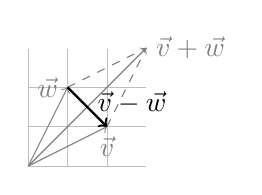
\begin{tikzpicture}
            \draw[step=0.5cm, gray!50, very thin](0,0) grid (1.49,1.49);
            \draw[thin, gray, ->] (0,0)--(1,0.5) node[below] {$\vec{v}$};
            \draw[thin, gray, ->] (0,0)--(0.5,1) node[left] {$\vec{w}$};
            \draw[thin, gray, dashed, -] (1,0.5)--(1.5,1.5);
            \draw[thin, gray, dashed, -] (0.5,1)--(1.5,1.5);
            \draw[thin, gray, ->] (0,0)--(1.5,1.5) node[right] at (1.5, 1.5) {$\vec{v}+\vec{w}$};
            \draw[thick, ->] (0.5,1)--(1,0.5) node[right] at (0.75, 0.80) {$\vec{v}-\vec{w}$};
      \end{tikzpicture}
\end{wrapfigure}
Using the second special case we can then construct \emph{vector subtraction}:
\[ \vec{v}-\vec{w} = \vec{v} + -1\cdot\vec{w}.  \]

This subtraction has a geometric interpretation such that $\vec{v}-\vec{w}$ is the vector pointing from the head of $\vec{w}$ to the head of $\vec{v}$ when both $\vec{v}$ and $\vec{w}$ are in canonical, or standard position.


With scalar multiplication, we can expand the commutativity and associativity of vector addition to the following:
\begin{thrm}
Suppose $\vec{v},\vec{w}\in\mathbb{R}^{n}$ are vectors and $c,d\in\mathbb{R}$ are scalars. Then the following properties hold:
      \begin{itemize}
            \item $c(\vec{v}+\vec{w}) = c\vec{v}+c\vec{w}$,
            \item $(c+d)\vec{v} = c\vec{v}+d\vec{v}$, and
            \item $c(d\vec{v}) = (cd)\vec{v}$.
      \end{itemize}
\end{thrm}

\begin{proof}
      To prove the first property, note that we can use the definition of vector addition to add the vectors inside the paranthesis, then use the definition of scalar multiplication as follows.
      \begin{align*}
            c(\vec{v}+\vec{w}) = c\cdot \left( \begin{smallmatrix} v_1+w_1 \\ v_2+w_2 \\ \vdots \\ v_n+w_n \end{smallmatrix} \right)
            =\left( \begin{smallmatrix} c(v_1+w_1) \\ c(v_2+w_2) \\ \vdots \\ c(v_n+w_n) \end{smallmatrix} \right)
            =\left( \begin{smallmatrix} cv_1+cw_1 \\ cv_2+cw_2 \\ \vdots \\ cv_n+cw_n \end{smallmatrix} \right)
            &=\left( \begin{smallmatrix} cv_1 \\ cv_2 \\ \vdots \\ cv_n \end{smallmatrix} \right) + \left( \begin{smallmatrix} cw_1 \\ cw_2 \\ \vdots \\ cw_n \end{smallmatrix} \right) \\
            &=c\cdot \left( \begin{smallmatrix} v_1 \\ v_2 \\ \vdots \\ v_n \end{smallmatrix} \right) + c\cdot \left( \begin{smallmatrix} w_1 \\ w_2 \\ \vdots \\ w_n \end{smallmatrix} \right)
            =c\vec{v}+c\vec{w}.
      \end{align*}
      The proofs of the other two properties would follow a similar pattern of reasoning that utilizes the definitions of vector addition and scalar multiplication.
\end{proof}

\end{document}
